\section {Setup} \label{sec:setup}

\subsection{\sw} \label{sec:SpaceWarps}
some words about \sw


\begin{figure}
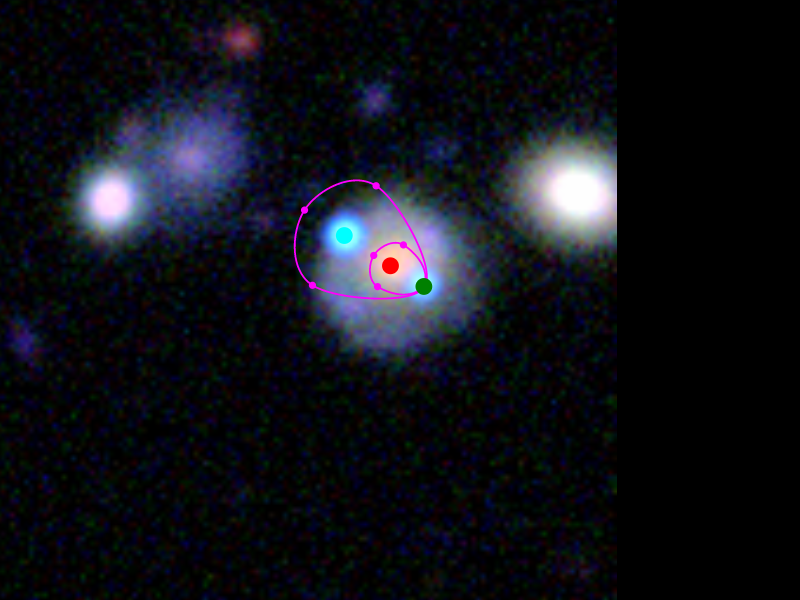
\includegraphics[height=.3\vsize]{fig/spag6941.png} \\
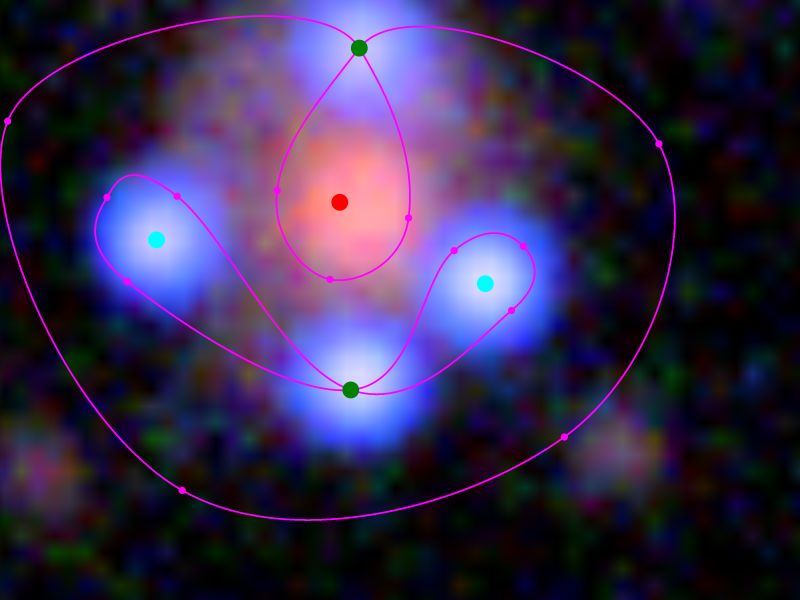
\includegraphics[height=.3\vsize]{fig/spag7022.png} \\
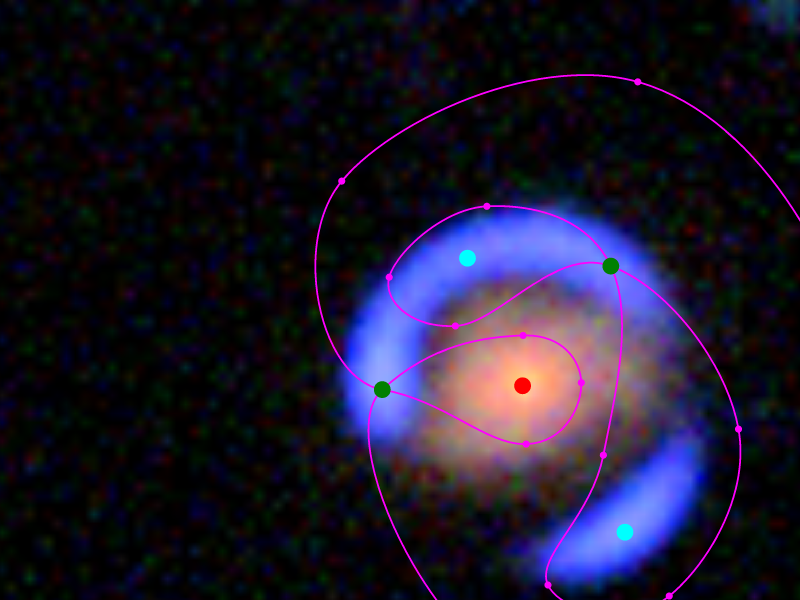
\includegraphics[height=.3\vsize]{fig/spag6919.png}
\caption{Examples of Spaghetti input.  The models from these appear
  later in Figures \ref{fig:6941}, \ref{fig:7022} and
  \ref{fig:6919}. \label{fig:input-spag}}
\end{figure}

\subsection{\spl} \label{sec:SpaghettiLens}



A saddle point is recognizable in a contour map because contours do
not loop around it, they tend to approach and then pull away.  There
is one contour ---the saddle-point contour--- that makes an X on the
saddle point itself.  A saddle point contour may not appear on a plot
(and Figure~\ref{fig:arriv} does not show one.  But we can tell from
the other contours where the saddle-point contour would be.



Give a guess for the maximum, minimum and saddle points.  Program
tries find $\kappa(x,y)$ that reproduces these properties exactly, and
looks reasonably like a galaxy.  Solution not unique, an ensemble
generated.

\hr

SpaghettiLens is build on top of GLASS \citep{Lubini2012}, that builds and improves upon PixeLens \citep{Saha2004}.
It provides a web based graphical user interface that allows to trace contours with the mouse and identify extremal points by clicking on the image.
\spl then tries to find a mass distribution $\kappa(x,y)$ that reproduces the input parameters.
Since there is no unique solution, \spl samples the solution space and produces an ensemble of solutions, as described in the paper \citep{Lubini2012}.
It provides direct visual feedback by rendering a synthetic image side by side the original image, such that users can directly compare the predictions of their model to the survey image.
It additinally provides plots of the modelled mass distribution and the contour lines of arrival time surface as feedback. 

Using this direct visual feedback, even unexperienced users can successfully model lenses using a iterative approach if they know what to look for.

The modelling process consitis of three basic steps:

\begin{enumerate}
  \item identify lensed images and separate them from other background light sources
  \item classify and order images accoring to arrival time. (local minima, maxima, saddlepoints)
  \item fine tune the arrangement, identify addidional external point masses influencing the result
\end{enumerate}

\spl assists volunteers with several features in this process.
Step 1 by supplying several images from several bands (not yet implemented in \sw).
Step 2 by restricting the user, only valid configuration can be entered, the odd number theorem\needcite is taken care of.
Step 3 by providing the visual feedback. Users can check the generated mass distribution and synthetic image.

Explanation:
Synthetic image: A rendering of the derivative of the arrival time for each pixel. This leads to a black and white image that reasonably looks like the visual appearace of the model.

Volunteers enter an assumed lens configuration and get a rendered synthetic image along with a reconstructed / simulated mass map and reconstructed / simulated contour lines.
This allows volunteers to directly see the effect of changing the parameters of the model and to iteratively approach a good solution.

In the next step, several volunteers can work together / exchange their ideas and models and try to improve previous modelling attempts by others.
This leads to a set of models organised in a branching, tree like structre for each model.
Volunteers then organise them selves to narrow down the different branches and come up with a few consensus models in the end.

\spl provides plug ins to support any data source. At the moment, a data link to \sw and to the MasterLens database\needcite are implemented.






\subsection{The simulated lenses} \label{sec:sims}

In order to estimate users performance, \sw included some simulated lensing configurations in their image set.

There are three kinds of simulated lenses:

\begin{itemize}
  \item {\em Quasar:\/} A singular elliptical isothermal plus constant
    external shear, with a circular Gaussian source.
  \item {\em Galaxy:\/} Lens as with quasar, but elliptical de
    Vaucouleurs source.
  \item {\em Galaxy:\/} Lens is circular NFW plus one dominant
    elliptical SIE and perturbating elliptical SIEs, source as with
    galaxy.
\end{itemize}
Lenses follow \cite{2001astro.ph..2341K,2001astro.ph..2340K}.

Parameters can be looked up in online supplement.


\subsection{The Test setup} \label{sec:testsetup}
We made use of this simulated lenses and further tested the volunteers abilities to model those simulated lensing images.

The testing was done with a small number of volunteers ($N_v=4$) and a set of simulated configurations ($N_{sim}=30$) chosen to represent some typical configurations.

Two tests were done on the models created by the volunteers:

\begin{enumerate}
  \item Correct identification of extremal points
  \item Reproduction of the mass distribution of the lens
\end{enumerate}

The first test required the volunteers to accomplish 2 tasks: First to identify and distinguish lensed images from background light sources.
Second to come up with a logical ordering of the arrival time of those lensed images.
It also tries to identify the problems volunteers encounter during modelling.

The second test compared the enclosed mass $\kappa(r)$ of the models and the simulations.
